\documentclass[1p]{elsarticle_modified}
%\bibliographystyle{elsarticle-num}

%\usepackage[colorlinks]{hyperref}
%\usepackage{abbrmath_seonhwa} %\Abb, \Ascr, \Acal ,\Abf, \Afrak
\usepackage{amsfonts}
\usepackage{amssymb}
\usepackage{amsmath}
\usepackage{amsthm}
\usepackage{scalefnt}
\usepackage{amsbsy}
\usepackage{kotex}
\usepackage{caption}
\usepackage{subfig}
\usepackage{color}
\usepackage{graphicx}
\usepackage{xcolor} %% white, black, red, green, blue, cyan, magenta, yellow
\usepackage{float}
\usepackage{setspace}
\usepackage{hyperref}

\usepackage{tikz}
\usetikzlibrary{arrows}

\usepackage{multirow}
\usepackage{array} % fixed length table
\usepackage{hhline}

%%%%%%%%%%%%%%%%%%%%%
\makeatletter
\renewcommand*\env@matrix[1][\arraystretch]{%
	\edef\arraystretch{#1}%
	\hskip -\arraycolsep
	\let\@ifnextchar\new@ifnextchar
	\array{*\c@MaxMatrixCols c}}
\makeatother %https://tex.stackexchange.com/questions/14071/how-can-i-increase-the-line-spacing-in-a-matrix
%%%%%%%%%%%%%%%

\usepackage[normalem]{ulem}

\newcommand{\msout}[1]{\ifmmode\text{\sout{\ensuremath{#1}}}\else\sout{#1}\fi}
%SOURCE: \msout is \stkout macro in https://tex.stackexchange.com/questions/20609/strikeout-in-math-mode

\newcommand{\cancel}[1]{
	\ifmmode
	{\color{red}\msout{#1}}
	\else
	{\color{red}\sout{#1}}
	\fi
}

\newcommand{\add}[1]{
	{\color{blue}\uwave{#1}}
}

\newcommand{\replace}[2]{
	\ifmmode
	{\color{red}\msout{#1}}{\color{blue}\uwave{#2}}
	\else
	{\color{red}\sout{#1}}{\color{blue}\uwave{#2}}
	\fi
}

\newcommand{\Sol}{\mathcal{S}} %segment
\newcommand{\D}{D} %diagram
\newcommand{\A}{\mathcal{A}} %arc


%%%%%%%%%%%%%%%%%%%%%%%%%%%%%5 test

\def\sl{\operatorname{\textup{SL}}(2,\Cbb)}
\def\psl{\operatorname{\textup{PSL}}(2,\Cbb)}
\def\quan{\mkern 1mu \triangleright \mkern 1mu}

\theoremstyle{definition}
\newtheorem{thm}{Theorem}[section]
\newtheorem{prop}[thm]{Proposition}
\newtheorem{lem}[thm]{Lemma}
\newtheorem{ques}[thm]{Question}
\newtheorem{cor}[thm]{Corollary}
\newtheorem{defn}[thm]{Definition}
\newtheorem{exam}[thm]{Example}
\newtheorem{rmk}[thm]{Remark}
\newtheorem{alg}[thm]{Algorithm}

\newcommand{\I}{\sqrt{-1}}
\begin{document}

%\begin{frontmatter}
%
%\title{Boundary parabolic representations of knots up to 8 crossings}
%
%%% Group authors per affiliation:
%\author{Yunhi Cho} 
%\address{Department of Mathematics, University of Seoul, Seoul, Korea}
%\ead{yhcho@uos.ac.kr}
%
%
%\author{Seonhwa Kim} %\fnref{s_kim}}
%\address{Center for Geometry and Physics, Institute for Basic Science, Pohang, 37673, Korea}
%\ead{ryeona17@ibs.re.kr}
%
%\author{Hyuk Kim}
%\address{Department of Mathematical Sciences, Seoul National University, Seoul 08826, Korea}
%\ead{hyukkim@snu.ac.kr}
%
%\author{Seokbeom Yoon}
%\address{Department of Mathematical Sciences, Seoul National University, Seoul, 08826,  Korea}
%\ead{sbyoon15@snu.ac.kr}
%
%\begin{abstract}
%We find all boundary parabolic representation of knots up to 8 crossings.
%
%\end{abstract}
%\begin{keyword}
%    \MSC[2010] 57M25 
%\end{keyword}
%
%\end{frontmatter}

%\linenumbers
%\tableofcontents
%
\newcommand\colored[1]{\textcolor{white}{\rule[-0.35ex]{0.8em}{1.4ex}}\kern-0.8em\color{red} #1}%
%\newcommand\colored[1]{\textcolor{white}{ #1}\kern-2.17ex	\textcolor{white}{ #1}\kern-1.81ex	\textcolor{white}{ #1}\kern-2.15ex\color{red}#1	}

{\Large $\underline{12a_{1084}~(K12a_{1084})}$}

\setlength{\tabcolsep}{10pt}
\renewcommand{\arraystretch}{1.6}
\vspace{1cm}\begin{tabular}{m{100pt}>{\centering\arraybackslash}m{274pt}}
\multirow{5}{120pt}{
	\centering
	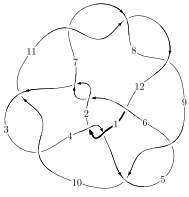
\includegraphics[width=112pt]{../../../GIT/diagram.site/Diagrams/png/1885_12a_1084.png}\\
\ \ \ A knot diagram\footnotemark}&
\allowdisplaybreaks
\textbf{Linearized knot diagam} \\
\cline{2-2}
 &
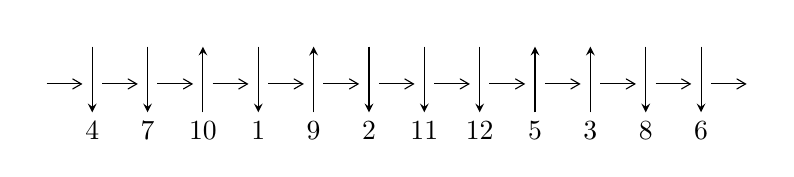
\begin{tikzpicture}[x=20pt, y=17pt]
	% nodes
	\node (C0) at (0, 0) {};
	\node (C1) at (1, 0) {};
	\node (C1U) at (1, +1) {};
	\node (C1D) at (1, -1) {4};

	\node (C2) at (2, 0) {};
	\node (C2U) at (2, +1) {};
	\node (C2D) at (2, -1) {7};

	\node (C3) at (3, 0) {};
	\node (C3U) at (3, +1) {};
	\node (C3D) at (3, -1) {10};

	\node (C4) at (4, 0) {};
	\node (C4U) at (4, +1) {};
	\node (C4D) at (4, -1) {1};

	\node (C5) at (5, 0) {};
	\node (C5U) at (5, +1) {};
	\node (C5D) at (5, -1) {9};

	\node (C6) at (6, 0) {};
	\node (C6U) at (6, +1) {};
	\node (C6D) at (6, -1) {2};

	\node (C7) at (7, 0) {};
	\node (C7U) at (7, +1) {};
	\node (C7D) at (7, -1) {11};

	\node (C8) at (8, 0) {};
	\node (C8U) at (8, +1) {};
	\node (C8D) at (8, -1) {12};

	\node (C9) at (9, 0) {};
	\node (C9U) at (9, +1) {};
	\node (C9D) at (9, -1) {5};

	\node (C10) at (10, 0) {};
	\node (C10U) at (10, +1) {};
	\node (C10D) at (10, -1) {3};

	\node (C11) at (11, 0) {};
	\node (C11U) at (11, +1) {};
	\node (C11D) at (11, -1) {8};

	\node (C12) at (12, 0) {};
	\node (C12U) at (12, +1) {};
	\node (C12D) at (12, -1) {6};
	\node (C13) at (13, 0) {};

	% arrows
	\draw[->,>={angle 60}]
	(C0) edge (C1) (C1) edge (C2) (C2) edge (C3) (C3) edge (C4) (C4) edge (C5) (C5) edge (C6) (C6) edge (C7) (C7) edge (C8) (C8) edge (C9) (C9) edge (C10) (C10) edge (C11) (C11) edge (C12) (C12) edge (C13) ;	\draw[->,>=stealth]
	(C1U) edge (C1D) (C2U) edge (C2D) (C3D) edge (C3U) (C4U) edge (C4D) (C5D) edge (C5U) (C6U) edge (C6D) (C7U) edge (C7D) (C8U) edge (C8D) (C9D) edge (C9U) (C10D) edge (C10U) (C11U) edge (C11D) (C12U) edge (C12D) ;
	\end{tikzpicture} \\
\hhline{~~} \\& 
\textbf{Solving Sequence} \\ \cline{2-2} 
 &
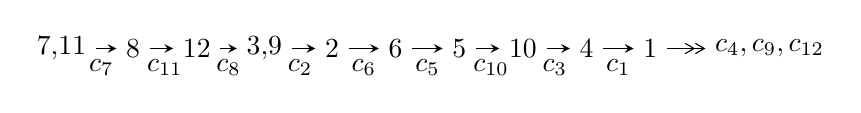
\begin{tikzpicture}[x=23pt, y=7pt]
	% node
	\node (A0) at (-1/8, 0) {7,11};
	\node (A1) at (1, 0) {8};
	\node (A2) at (2, 0) {12};
	\node (A3) at (49/16, 0) {3,9};
	\node (A4) at (33/8, 0) {2};
	\node (A5) at (41/8, 0) {6};
	\node (A6) at (49/8, 0) {5};
	\node (A7) at (57/8, 0) {10};
	\node (A8) at (65/8, 0) {4};
	\node (A9) at (73/8, 0) {1};
	\node (C1) at (1/2, -1) {$c_{7}$};
	\node (C2) at (3/2, -1) {$c_{11}$};
	\node (C3) at (5/2, -1) {$c_{8}$};
	\node (C4) at (29/8, -1) {$c_{2}$};
	\node (C5) at (37/8, -1) {$c_{6}$};
	\node (C6) at (45/8, -1) {$c_{5}$};
	\node (C7) at (53/8, -1) {$c_{10}$};
	\node (C8) at (61/8, -1) {$c_{3}$};
	\node (C9) at (69/8, -1) {$c_{1}$};
	\node (A10) at (11, 0) {$c_{4},c_{9},c_{12}$};

	% edge
	\draw[->,>=stealth]	
	(A0) edge (A1) (A1) edge (A2) (A2) edge (A3) (A3) edge (A4) (A4) edge (A5) (A5) edge (A6) (A6) edge (A7) (A7) edge (A8) (A8) edge (A9) ;
	\draw[->>,>={angle 60}]	
	(A9) edge (A10);
\end{tikzpicture} \\ 

\end{tabular} \\

\footnotetext{
The image of knot diagram is generated by the software ``\textbf{Draw programme}" developed by Andrew Bartholomew(\url{http://www.layer8.co.uk/maths/draw/index.htm\#Running-draw}), where we modified some parts for our purpose(\url{https://github.com/CATsTAILs/LinksPainter}).
}\phantom \\ \newline 
\centering \textbf{Ideals for irreducible components\footnotemark of $X_{\text{par}}$} 
 
\begin{align*}
I^u_{1}&=\langle 
5.41095\times10^{226} u^{98}-5.69026\times10^{226} u^{97}+\cdots+5.42259\times10^{227} b-1.90870\times10^{229},\\
\phantom{I^u_{1}}&\phantom{= \langle  }-2.17596\times10^{230} u^{98}+3.39515\times10^{230} u^{97}+\cdots+5.43886\times10^{230} a+4.44885\times10^{233},\\
\phantom{I^u_{1}}&\phantom{= \langle  }u^{99}-4 u^{98}+\cdots+2545 u+1003\rangle \\
I^u_{2}&=\langle 
2996823 u^{26}+3522809 u^{25}+\cdots+792677 b-4094869,\\
\phantom{I^u_{2}}&\phantom{= \langle  }-533686 u^{26}+1883904 u^{25}+\cdots+792677 a+5658204,\;u^{27}+3 u^{26}+\cdots+5 u-1\rangle \\
\\
\end{align*}
\raggedright * 2 irreducible components of $\dim_{\mathbb{C}}=0$, with total 126 representations.\\
\footnotetext{All coefficients of polynomials are rational numbers. But the coefficients are sometimes approximated in decimal forms when there is not enough margin.}
\newpage
\renewcommand{\arraystretch}{1}
\centering \section*{I. $I^u_{1}= \langle 5.41\times10^{226} u^{98}-5.69\times10^{226} u^{97}+\cdots+5.42\times10^{227} b-1.91\times10^{229},\;-2.18\times10^{230} u^{98}+3.40\times10^{230} u^{97}+\cdots+5.44\times10^{230} a+4.45\times10^{233},\;u^{99}-4 u^{98}+\cdots+2545 u+1003 \rangle$}
\flushleft \textbf{(i) Arc colorings}\\
\begin{tabular}{m{7pt} m{180pt} m{7pt} m{180pt} }
\flushright $a_{7}=$&$\begin{pmatrix}1\\0\end{pmatrix}$ \\
\flushright $a_{11}=$&$\begin{pmatrix}0\\u\end{pmatrix}$ \\
\flushright $a_{8}=$&$\begin{pmatrix}1\\u^2\end{pmatrix}$ \\
\flushright $a_{12}=$&$\begin{pmatrix}- u\\- u^3+u\end{pmatrix}$ \\
\flushright $a_{3}=$&$\begin{pmatrix}0.400077 u^{98}-0.624239 u^{97}+\cdots-1633.59 u-817.975\\-0.0997853 u^{98}+0.104936 u^{97}+\cdots+340.396 u+35.1990\end{pmatrix}$ \\
\flushright $a_{9}=$&$\begin{pmatrix}- u^2+1\\- u^4+2 u^2\end{pmatrix}$ \\
\flushright $a_{2}=$&$\begin{pmatrix}0.300292 u^{98}-0.519303 u^{97}+\cdots-1293.20 u-782.776\\-0.0997853 u^{98}+0.104936 u^{97}+\cdots+340.396 u+35.1990\end{pmatrix}$ \\
\flushright $a_{6}=$&$\begin{pmatrix}0.0548331 u^{98}-0.912289 u^{97}+\cdots+1474.97 u+778.578\\0.0336398 u^{98}-0.236589 u^{97}+\cdots+237.616 u+235.987\end{pmatrix}$ \\
\flushright $a_{5}=$&$\begin{pmatrix}0.0408862 u^{98}-1.05461 u^{97}+\cdots+1912.99 u+1025.59\\0.0737455 u^{98}-0.370751 u^{97}+\cdots+271.358 u+328.673\end{pmatrix}$ \\
\flushright $a_{10}=$&$\begin{pmatrix}-0.695680 u^{98}+1.69937 u^{97}+\cdots+1342.50 u+887.962\\-0.590927 u^{98}+1.84609 u^{97}+\cdots+488.653 u-21.2569\end{pmatrix}$ \\
\flushright $a_{4}=$&$\begin{pmatrix}1.75208 u^{98}-4.12027 u^{97}+\cdots-3777.53 u-756.930\\1.86946 u^{98}-4.33276 u^{97}+\cdots-4177.35 u-1429.35\end{pmatrix}$ \\
\flushright $a_{1}=$&$\begin{pmatrix}1.75093 u^{98}-3.19905 u^{97}+\cdots-6038.12 u-2076.45\\0.485526 u^{98}-0.641300 u^{97}+\cdots-2274.29 u-1238.76\end{pmatrix}$\\&\end{tabular}
\flushleft \textbf{(ii) Obstruction class $= -1$}\\~\\
\flushleft \textbf{(iii) Cusp Shapes $= -0.887479 u^{98}+2.43148 u^{97}+\cdots+1143.39 u+1477.84$}\\~\\
\newpage\renewcommand{\arraystretch}{1}
\flushleft \textbf{(iv) u-Polynomials at the component}\newline \\
\begin{tabular}{m{50pt}|m{274pt}}
Crossings & \hspace{64pt}u-Polynomials at each crossing \\
\hline $$\begin{aligned}c_{1},c_{4}\end{aligned}$$&$\begin{aligned}
&u^{99}-8 u^{98}+\cdots+19 u-1
\end{aligned}$\\
\hline $$\begin{aligned}c_{2},c_{6}\end{aligned}$$&$\begin{aligned}
&u^{99}-2 u^{98}+\cdots-21137 u-8401
\end{aligned}$\\
\hline $$\begin{aligned}c_{3},c_{10}\end{aligned}$$&$\begin{aligned}
&u^{99}+u^{98}+\cdots-17146 u-20252
\end{aligned}$\\
\hline $$\begin{aligned}c_{5},c_{9}\end{aligned}$$&$\begin{aligned}
&u^{99}-3 u^{98}+\cdots-1873 u-577
\end{aligned}$\\
\hline $$\begin{aligned}c_{7},c_{8},c_{11}\end{aligned}$$&$\begin{aligned}
&u^{99}+4 u^{98}+\cdots+2545 u-1003
\end{aligned}$\\
\hline $$\begin{aligned}c_{12}\end{aligned}$$&$\begin{aligned}
&u^{99}+2 u^{98}+\cdots-23310064 u-2254444
\end{aligned}$\\
\hline
\end{tabular}\\~\\
\newpage\renewcommand{\arraystretch}{1}
\flushleft \textbf{(v) Riley Polynomials at the component}\newline \\
\begin{tabular}{m{50pt}|m{274pt}}
Crossings & \hspace{64pt}Riley Polynomials at each crossing \\
\hline $$\begin{aligned}c_{1},c_{4}\end{aligned}$$&$\begin{aligned}
&y^{99}+56 y^{98}+\cdots+87 y-1
\end{aligned}$\\
\hline $$\begin{aligned}c_{2},c_{6}\end{aligned}$$&$\begin{aligned}
&y^{99}-80 y^{98}+\cdots-692503643 y-70576801
\end{aligned}$\\
\hline $$\begin{aligned}c_{3},c_{10}\end{aligned}$$&$\begin{aligned}
&y^{99}+95 y^{98}+\cdots+3720826236 y-410143504
\end{aligned}$\\
\hline $$\begin{aligned}c_{5},c_{9}\end{aligned}$$&$\begin{aligned}
&y^{99}+71 y^{98}+\cdots-12786351 y-332929
\end{aligned}$\\
\hline $$\begin{aligned}c_{7},c_{8},c_{11}\end{aligned}$$&$\begin{aligned}
&y^{99}-120 y^{98}+\cdots+48189789 y-1006009
\end{aligned}$\\
\hline $$\begin{aligned}c_{12}\end{aligned}$$&$\begin{aligned}
&y^{99}-42 y^{98}+\cdots+169128066365000 y-5082517749136
\end{aligned}$\\
\hline
\end{tabular}\\~\\
\newpage\flushleft \textbf{(vi) Complex Volumes and Cusp Shapes}
$$\begin{array}{c|c|c}  
\text{Solutions to }I^u_{1}& \I (\text{vol} + \sqrt{-1}CS) & \text{Cusp shape}\\
 \hline 
\begin{aligned}
u &= \phantom{-}0.671582 + 0.666153 I \\
a &= -0.81851 - 1.26445 I \\
b &= \phantom{-}1.39390 + 0.42952 I\end{aligned}
 & -3.01360 - 7.08917 I & \phantom{-0.000000 } 0 \\ \hline\begin{aligned}
u &= \phantom{-}0.671582 - 0.666153 I \\
a &= -0.81851 + 1.26445 I \\
b &= \phantom{-}1.39390 - 0.42952 I\end{aligned}
 & -3.01360 + 7.08917 I & \phantom{-0.000000 } 0 \\ \hline\begin{aligned}
u &= \phantom{-}0.625140 + 0.686233 I \\
a &= \phantom{-}0.834216 + 0.986532 I \\
b &= -1.391950 - 0.146302 I\end{aligned}
 & -5.26496 - 2.40033 I & \phantom{-0.000000 } 0 \\ \hline\begin{aligned}
u &= \phantom{-}0.625140 - 0.686233 I \\
a &= \phantom{-}0.834216 - 0.986532 I \\
b &= -1.391950 + 0.146302 I\end{aligned}
 & -5.26496 + 2.40033 I & \phantom{-0.000000 } 0 \\ \hline\begin{aligned}
u &= \phantom{-}0.422701 + 0.807441 I \\
a &= -1.30778 - 0.63709 I \\
b &= \phantom{-}1.236250 - 0.119711 I\end{aligned}
 & -2.18481 + 2.18176 I & \phantom{-0.000000 } 0 \\ \hline\begin{aligned}
u &= \phantom{-}0.422701 - 0.807441 I \\
a &= -1.30778 + 0.63709 I \\
b &= \phantom{-}1.236250 + 0.119711 I\end{aligned}
 & -2.18481 - 2.18176 I & \phantom{-0.000000 } 0 \\ \hline\begin{aligned}
u &= -0.896243 + 0.006019 I \\
a &= -0.228443 + 0.713126 I \\
b &= -0.836938 - 0.795713 I\end{aligned}
 & \phantom{-}1.52179 - 2.96179 I & \phantom{-0.000000 } 0 \\ \hline\begin{aligned}
u &= -0.896243 - 0.006019 I \\
a &= -0.228443 - 0.713126 I \\
b &= -0.836938 + 0.795713 I\end{aligned}
 & \phantom{-}1.52179 + 2.96179 I & \phantom{-0.000000 } 0 \\ \hline\begin{aligned}
u &= \phantom{-}0.561471 + 0.662733 I \\
a &= \phantom{-}0.709135 + 1.118490 I \\
b &= -1.366860 - 0.093390 I\end{aligned}
 & -5.13995 - 2.31729 I & \phantom{-0.000000 } 0 \\ \hline\begin{aligned}
u &= \phantom{-}0.561471 - 0.662733 I \\
a &= \phantom{-}0.709135 - 1.118490 I \\
b &= -1.366860 + 0.093390 I\end{aligned}
 & -5.13995 + 2.31729 I & \phantom{-0.000000 } 0\\
 \hline 
 \end{array}$$\newpage$$\begin{array}{c|c|c}  
\text{Solutions to }I^u_{1}& \I (\text{vol} + \sqrt{-1}CS) & \text{Cusp shape}\\
 \hline 
\begin{aligned}
u &= \phantom{-}0.632131 + 0.587585 I \\
a &= -0.128876 + 0.582565 I \\
b &= -1.121870 - 0.038053 I\end{aligned}
 & -4.62953 - 2.16317 I & \phantom{-0.000000 } 0 \\ \hline\begin{aligned}
u &= \phantom{-}0.632131 - 0.587585 I \\
a &= -0.128876 - 0.582565 I \\
b &= -1.121870 + 0.038053 I\end{aligned}
 & -4.62953 + 2.16317 I & \phantom{-0.000000 } 0 \\ \hline\begin{aligned}
u &= \phantom{-}1.15287\phantom{ +0.000000I} \\
a &= -0.329540\phantom{ +0.000000I} \\
b &= -0.490126\phantom{ +0.000000I}\end{aligned}
 & -2.39809\phantom{ +0.000000I} & \phantom{-0.000000 } 0 \\ \hline\begin{aligned}
u &= -0.647182 + 0.484954 I \\
a &= \phantom{-}0.81717 - 1.19305 I \\
b &= -0.064411 + 0.544461 I\end{aligned}
 & -5.31603 + 1.89708 I & \phantom{-0.000000 } 0 \\ \hline\begin{aligned}
u &= -0.647182 - 0.484954 I \\
a &= \phantom{-}0.81717 + 1.19305 I \\
b &= -0.064411 - 0.544461 I\end{aligned}
 & -5.31603 - 1.89708 I & \phantom{-0.000000 } 0 \\ \hline\begin{aligned}
u &= -0.656533 + 0.429069 I \\
a &= -0.31014 + 1.49332 I \\
b &= \phantom{-}0.055583 - 1.009320 I\end{aligned}
 & -2.21186 + 7.67640 I & \phantom{-0.000000 } 0 \\ \hline\begin{aligned}
u &= -0.656533 - 0.429069 I \\
a &= -0.31014 - 1.49332 I \\
b &= \phantom{-}0.055583 + 1.009320 I\end{aligned}
 & -2.21186 - 7.67640 I & \phantom{-0.000000 } 0 \\ \hline\begin{aligned}
u &= -0.884666 + 0.838961 I \\
a &= \phantom{-}0.548928 - 1.096780 I \\
b &= -1.38567 + 0.40064 I\end{aligned}
 & -6.8912 + 12.6306 I & \phantom{-0.000000 } 0 \\ \hline\begin{aligned}
u &= -0.884666 - 0.838961 I \\
a &= \phantom{-}0.548928 + 1.096780 I \\
b &= -1.38567 - 0.40064 I\end{aligned}
 & -6.8912 - 12.6306 I & \phantom{-0.000000 } 0 \\ \hline\begin{aligned}
u &= \phantom{-}0.389722 + 0.629908 I \\
a &= -0.832777 + 0.668407 I \\
b &= \phantom{-}0.292539 - 0.596900 I\end{aligned}
 & \phantom{-}0.39264 - 3.39831 I & \phantom{-0.000000 } 0\\
 \hline 
 \end{array}$$\newpage$$\begin{array}{c|c|c}  
\text{Solutions to }I^u_{1}& \I (\text{vol} + \sqrt{-1}CS) & \text{Cusp shape}\\
 \hline 
\begin{aligned}
u &= \phantom{-}0.389722 - 0.629908 I \\
a &= -0.832777 - 0.668407 I \\
b &= \phantom{-}0.292539 + 0.596900 I\end{aligned}
 & \phantom{-}0.39264 + 3.39831 I & \phantom{-0.000000 } 0 \\ \hline\begin{aligned}
u &= \phantom{-}0.459085 + 0.568866 I \\
a &= -0.162137 + 0.715721 I \\
b &= \phantom{-}0.927472 - 0.541537 I\end{aligned}
 & -1.47108 + 3.63726 I & \phantom{-0.000000 } 0 \\ \hline\begin{aligned}
u &= \phantom{-}0.459085 - 0.568866 I \\
a &= -0.162137 - 0.715721 I \\
b &= \phantom{-}0.927472 + 0.541537 I\end{aligned}
 & -1.47108 - 3.63726 I & \phantom{-0.000000 } 0 \\ \hline\begin{aligned}
u &= \phantom{-}0.565793 + 0.435926 I \\
a &= \phantom{-}1.24415 - 1.19701 I \\
b &= \phantom{-}1.048280 + 0.361406 I\end{aligned}
 & -1.81044 - 7.03502 I & \phantom{-0.000000 } 0 \\ \hline\begin{aligned}
u &= \phantom{-}0.565793 - 0.435926 I \\
a &= \phantom{-}1.24415 + 1.19701 I \\
b &= \phantom{-}1.048280 - 0.361406 I\end{aligned}
 & -1.81044 + 7.03502 I & \phantom{-0.000000 } 0 \\ \hline\begin{aligned}
u &= \phantom{-}0.509382 + 0.498338 I \\
a &= \phantom{-}0.132878 - 1.139320 I \\
b &= \phantom{-}0.344177 + 0.527838 I\end{aligned}
 & -0.086668 - 0.470961 I & \phantom{-0.000000 } 0 \\ \hline\begin{aligned}
u &= \phantom{-}0.509382 - 0.498338 I \\
a &= \phantom{-}0.132878 + 1.139320 I \\
b &= \phantom{-}0.344177 - 0.527838 I\end{aligned}
 & -0.086668 + 0.470961 I & \phantom{-0.000000 } 0 \\ \hline\begin{aligned}
u &= -0.232634 + 1.269800 I \\
a &= \phantom{-}0.987311 - 0.040384 I \\
b &= -1.269770 - 0.132436 I\end{aligned}
 & -4.83968 - 6.00928 I & \phantom{-0.000000 } 0 \\ \hline\begin{aligned}
u &= -0.232634 - 1.269800 I \\
a &= \phantom{-}0.987311 + 0.040384 I \\
b &= -1.269770 + 0.132436 I\end{aligned}
 & -4.83968 + 6.00928 I & \phantom{-0.000000 } 0 \\ \hline\begin{aligned}
u &= -0.626540 + 0.273548 I \\
a &= \phantom{-}0.93551 - 2.09001 I \\
b &= -1.234250 + 0.462376 I\end{aligned}
 & -8.25997 + 1.73585 I & \phantom{-0.000000 } 0\\
 \hline 
 \end{array}$$\newpage$$\begin{array}{c|c|c}  
\text{Solutions to }I^u_{1}& \I (\text{vol} + \sqrt{-1}CS) & \text{Cusp shape}\\
 \hline 
\begin{aligned}
u &= -0.626540 - 0.273548 I \\
a &= \phantom{-}0.93551 + 2.09001 I \\
b &= -1.234250 - 0.462376 I\end{aligned}
 & -8.25997 - 1.73585 I & \phantom{-0.000000 } 0 \\ \hline\begin{aligned}
u &= -0.362556 + 0.575051 I \\
a &= -1.68279 - 0.01512 I \\
b &= -0.143843 + 0.295187 I\end{aligned}
 & -1.23465 - 4.31084 I & \phantom{-0.000000 } 0 \\ \hline\begin{aligned}
u &= -0.362556 - 0.575051 I \\
a &= -1.68279 + 0.01512 I \\
b &= -0.143843 - 0.295187 I\end{aligned}
 & -1.23465 + 4.31084 I & \phantom{-0.000000 } 0 \\ \hline\begin{aligned}
u &= \phantom{-}0.676867 + 0.044621 I \\
a &= \phantom{-}0.94289 + 1.18081 I \\
b &= \phantom{-}0.469702 + 0.239598 I\end{aligned}
 & \phantom{-}0.632736 + 0.678056 I & \phantom{-0.000000 } 0 \\ \hline\begin{aligned}
u &= \phantom{-}0.676867 - 0.044621 I \\
a &= \phantom{-}0.94289 - 1.18081 I \\
b &= \phantom{-}0.469702 - 0.239598 I\end{aligned}
 & \phantom{-}0.632736 - 0.678056 I & \phantom{-0.000000 } 0 \\ \hline\begin{aligned}
u &= -0.647432 + 0.189841 I \\
a &= -0.72737 + 1.72532 I \\
b &= \phantom{-}1.49112 - 0.35700 I\end{aligned}
 & -7.01581 - 2.36185 I & \phantom{-0.000000 } 0 \\ \hline\begin{aligned}
u &= -0.647432 - 0.189841 I \\
a &= -0.72737 - 1.72532 I \\
b &= \phantom{-}1.49112 + 0.35700 I\end{aligned}
 & -7.01581 + 2.36185 I & \phantom{-0.000000 } 0 \\ \hline\begin{aligned}
u &= \phantom{-}1.339350 + 0.111965 I \\
a &= \phantom{-}0.148541 + 0.088908 I \\
b &= -0.442208 + 0.756719 I\end{aligned}
 & -1.48538 - 0.70299 I & \phantom{-0.000000 } 0 \\ \hline\begin{aligned}
u &= \phantom{-}1.339350 - 0.111965 I \\
a &= \phantom{-}0.148541 - 0.088908 I \\
b &= -0.442208 - 0.756719 I\end{aligned}
 & -1.48538 + 0.70299 I & \phantom{-0.000000 } 0 \\ \hline\begin{aligned}
u &= -1.42141 + 0.18001 I \\
a &= \phantom{-}0.259621 + 0.430934 I \\
b &= \phantom{-}0.296118 - 0.499010 I\end{aligned}
 & -6.11710 + 2.82126 I & \phantom{-0.000000 } 0\\
 \hline 
 \end{array}$$\newpage$$\begin{array}{c|c|c}  
\text{Solutions to }I^u_{1}& \I (\text{vol} + \sqrt{-1}CS) & \text{Cusp shape}\\
 \hline 
\begin{aligned}
u &= -1.42141 - 0.18001 I \\
a &= \phantom{-}0.259621 - 0.430934 I \\
b &= \phantom{-}0.296118 + 0.499010 I\end{aligned}
 & -6.11710 - 2.82126 I & \phantom{-0.000000 } 0 \\ \hline\begin{aligned}
u &= -0.502166 + 0.238090 I \\
a &= -0.996833 - 0.817909 I \\
b &= -0.908820 + 0.518858 I\end{aligned}
 & \phantom{-}2.03936 + 3.39507 I & \phantom{-}0.73878 - 7.34492 I \\ \hline\begin{aligned}
u &= -0.502166 - 0.238090 I \\
a &= -0.996833 + 0.817909 I \\
b &= -0.908820 - 0.518858 I\end{aligned}
 & \phantom{-}2.03936 - 3.39507 I & \phantom{-}0.73878 + 7.34492 I \\ \hline\begin{aligned}
u &= -0.486584 + 0.268353 I \\
a &= \phantom{-}1.16169 - 3.08951 I \\
b &= -1.136470 - 0.000745 I\end{aligned}
 & -7.76651 + 0.21651 I & -10.72357 + 1.56326 I \\ \hline\begin{aligned}
u &= -0.486584 - 0.268353 I \\
a &= \phantom{-}1.16169 + 3.08951 I \\
b &= -1.136470 + 0.000745 I\end{aligned}
 & -7.76651 - 0.21651 I & -10.72357 - 1.56326 I \\ \hline\begin{aligned}
u &= -1.44027 + 0.22382 I \\
a &= -0.490873 - 0.025787 I \\
b &= \phantom{-}0.225206 + 0.508462 I\end{aligned}
 & -5.48236 + 6.48741 I & \phantom{-0.000000 } 0 \\ \hline\begin{aligned}
u &= -1.44027 - 0.22382 I \\
a &= -0.490873 + 0.025787 I \\
b &= \phantom{-}0.225206 - 0.508462 I\end{aligned}
 & -5.48236 - 6.48741 I & \phantom{-0.000000 } 0 \\ \hline\begin{aligned}
u &= -0.490936 + 0.178178 I \\
a &= \phantom{-}0.24238 + 3.11516 I \\
b &= \phantom{-}1.382040 - 0.014841 I\end{aligned}
 & -6.44341 + 3.68086 I & -13.6904 - 4.8990 I \\ \hline\begin{aligned}
u &= -0.490936 - 0.178178 I \\
a &= \phantom{-}0.24238 - 3.11516 I \\
b &= \phantom{-}1.382040 + 0.014841 I\end{aligned}
 & -6.44341 - 3.68086 I & -13.6904 + 4.8990 I \\ \hline\begin{aligned}
u &= -1.48618 + 0.00613 I \\
a &= \phantom{-}0.098528 + 0.813606 I \\
b &= \phantom{-}0.315796 - 0.762481 I\end{aligned}
 & -6.09592 + 1.64565 I & \phantom{-0.000000 } 0\\
 \hline 
 \end{array}$$\newpage$$\begin{array}{c|c|c}  
\text{Solutions to }I^u_{1}& \I (\text{vol} + \sqrt{-1}CS) & \text{Cusp shape}\\
 \hline 
\begin{aligned}
u &= -1.48618 - 0.00613 I \\
a &= \phantom{-}0.098528 - 0.813606 I \\
b &= \phantom{-}0.315796 + 0.762481 I\end{aligned}
 & -6.09592 - 1.64565 I & \phantom{-0.000000 } 0 \\ \hline\begin{aligned}
u &= -0.178980 + 0.439864 I \\
a &= \phantom{-}1.056880 + 0.579358 I \\
b &= -0.531876 - 0.756279 I\end{aligned}
 & \phantom{-}3.23925 - 1.18451 I & \phantom{-}3.17617 + 1.25796 I \\ \hline\begin{aligned}
u &= -0.178980 - 0.439864 I \\
a &= \phantom{-}1.056880 - 0.579358 I \\
b &= -0.531876 + 0.756279 I\end{aligned}
 & \phantom{-}3.23925 + 1.18451 I & \phantom{-}3.17617 - 1.25796 I \\ \hline\begin{aligned}
u &= \phantom{-}0.465205 + 0.093431 I \\
a &= -0.07254 + 2.27543 I \\
b &= \phantom{-}0.204842 - 1.190100 I\end{aligned}
 & \phantom{-}1.36006 - 1.43745 I & -12.0554 + 7.7332 I \\ \hline\begin{aligned}
u &= \phantom{-}0.465205 - 0.093431 I \\
a &= -0.07254 - 2.27543 I \\
b &= \phantom{-}0.204842 + 1.190100 I\end{aligned}
 & \phantom{-}1.36006 + 1.43745 I & -12.0554 - 7.7332 I \\ \hline\begin{aligned}
u &= \phantom{-}1.54191 + 0.03849 I \\
a &= -0.790361 + 0.168672 I \\
b &= -1.305740 - 0.260764 I\end{aligned}
 & -4.84551 - 4.27483 I & \phantom{-0.000000 } 0 \\ \hline\begin{aligned}
u &= \phantom{-}1.54191 - 0.03849 I \\
a &= -0.790361 - 0.168672 I \\
b &= -1.305740 + 0.260764 I\end{aligned}
 & -4.84551 + 4.27483 I & \phantom{-0.000000 } 0 \\ \hline\begin{aligned}
u &= \phantom{-}1.55153\phantom{ +0.000000I} \\
a &= \phantom{-}0.691794\phantom{ +0.000000I} \\
b &= \phantom{-}1.41813\phantom{ +0.000000I}\end{aligned}
 & -8.58947\phantom{ +0.000000I} & \phantom{-0.000000 } 0 \\ \hline\begin{aligned}
u &= \phantom{-}1.56140 + 0.07649 I \\
a &= -0.27530 + 1.40786 I \\
b &= -1.140370 - 0.297190 I\end{aligned}
 & -14.8432 - 1.4473 I & \phantom{-0.000000 } 0 \\ \hline\begin{aligned}
u &= \phantom{-}1.56140 - 0.07649 I \\
a &= -0.27530 - 1.40786 I \\
b &= -1.140370 + 0.297190 I\end{aligned}
 & -14.8432 + 1.4473 I & \phantom{-0.000000 } 0\\
 \hline 
 \end{array}$$\newpage$$\begin{array}{c|c|c}  
\text{Solutions to }I^u_{1}& \I (\text{vol} + \sqrt{-1}CS) & \text{Cusp shape}\\
 \hline 
\begin{aligned}
u &= -1.56585 + 0.01882 I \\
a &= -0.050219 - 0.867231 I \\
b &= \phantom{-}0.22809 + 1.70840 I\end{aligned}
 & -5.74012 + 1.79605 I & \phantom{-0.000000 } 0 \\ \hline\begin{aligned}
u &= -1.56585 - 0.01882 I \\
a &= -0.050219 + 0.867231 I \\
b &= \phantom{-}0.22809 - 1.70840 I\end{aligned}
 & -5.74012 - 1.79605 I & \phantom{-0.000000 } 0 \\ \hline\begin{aligned}
u &= \phantom{-}1.56534 + 0.05266 I \\
a &= \phantom{-}0.653824 - 1.146550 I \\
b &= \phantom{-}1.43207 + 0.25279 I\end{aligned}
 & -13.5869 - 4.5151 I & \phantom{-0.000000 } 0 \\ \hline\begin{aligned}
u &= \phantom{-}1.56534 - 0.05266 I \\
a &= \phantom{-}0.653824 + 1.146550 I \\
b &= \phantom{-}1.43207 - 0.25279 I\end{aligned}
 & -13.5869 + 4.5151 I & \phantom{-0.000000 } 0 \\ \hline\begin{aligned}
u &= -0.431395\phantom{ +0.000000I} \\
a &= \phantom{-}1.13469\phantom{ +0.000000I} \\
b &= \phantom{-}0.946642\phantom{ +0.000000I}\end{aligned}
 & -1.70568\phantom{ +0.000000I} & -3.51530\phantom{ +0.000000I} \\ \hline\begin{aligned}
u &= -1.05293 + 1.16373 I \\
a &= -0.552771 + 0.656982 I \\
b &= \phantom{-}1.295040 - 0.191585 I\end{aligned}
 & -9.47040 + 4.51904 I & \phantom{-0.000000 } 0 \\ \hline\begin{aligned}
u &= -1.05293 - 1.16373 I \\
a &= -0.552771 - 0.656982 I \\
b &= \phantom{-}1.295040 + 0.191585 I\end{aligned}
 & -9.47040 - 4.51904 I & \phantom{-0.000000 } 0 \\ \hline\begin{aligned}
u &= \phantom{-}0.284081 + 0.308258 I \\
a &= -0.439234 - 1.143360 I \\
b &= \phantom{-}0.214478 + 0.317345 I\end{aligned}
 & -0.189428 - 0.841299 I & -4.65351 + 7.98617 I \\ \hline\begin{aligned}
u &= \phantom{-}0.284081 - 0.308258 I \\
a &= -0.439234 + 1.143360 I \\
b &= \phantom{-}0.214478 - 0.317345 I\end{aligned}
 & -0.189428 + 0.841299 I & -4.65351 - 7.98617 I \\ \hline\begin{aligned}
u &= -1.57655 + 0.11657 I \\
a &= \phantom{-}1.105590 + 0.283380 I \\
b &= \phantom{-}1.302210 - 0.195925 I\end{aligned}
 & -9.12473 + 8.98920 I & \phantom{-0.000000 } 0\\
 \hline 
 \end{array}$$\newpage$$\begin{array}{c|c|c}  
\text{Solutions to }I^u_{1}& \I (\text{vol} + \sqrt{-1}CS) & \text{Cusp shape}\\
 \hline 
\begin{aligned}
u &= -1.57655 - 0.11657 I \\
a &= \phantom{-}1.105590 - 0.283380 I \\
b &= \phantom{-}1.302210 + 0.195925 I\end{aligned}
 & -9.12473 - 8.98920 I & \phantom{-0.000000 } 0 \\ \hline\begin{aligned}
u &= -1.57232 + 0.17577 I \\
a &= -0.525222 - 0.887076 I \\
b &= -1.49086 + 0.22367 I\end{aligned}
 & -12.31410 + 5.28789 I & \phantom{-0.000000 } 0 \\ \hline\begin{aligned}
u &= -1.57232 - 0.17577 I \\
a &= -0.525222 + 0.887076 I \\
b &= -1.49086 - 0.22367 I\end{aligned}
 & -12.31410 - 5.28789 I & \phantom{-0.000000 } 0 \\ \hline\begin{aligned}
u &= \phantom{-}1.60156 + 0.07631 I \\
a &= -0.080976 + 1.002640 I \\
b &= -1.39765 - 0.86415 I\end{aligned}
 & -15.9884 - 3.0243 I & \phantom{-0.000000 } 0 \\ \hline\begin{aligned}
u &= \phantom{-}1.60156 - 0.07631 I \\
a &= -0.080976 - 1.002640 I \\
b &= -1.39765 + 0.86415 I\end{aligned}
 & -15.9884 + 3.0243 I & \phantom{-0.000000 } 0 \\ \hline\begin{aligned}
u &= \phantom{-}1.60206 + 0.11818 I \\
a &= \phantom{-}0.083430 - 0.863594 I \\
b &= \phantom{-}0.13553 + 1.48784 I\end{aligned}
 & -9.94507 - 9.67187 I & \phantom{-0.000000 } 0 \\ \hline\begin{aligned}
u &= \phantom{-}1.60206 - 0.11818 I \\
a &= \phantom{-}0.083430 + 0.863594 I \\
b &= \phantom{-}0.13553 - 1.48784 I\end{aligned}
 & -9.94507 + 9.67187 I & \phantom{-0.000000 } 0 \\ \hline\begin{aligned}
u &= \phantom{-}1.60254 + 0.12020 I \\
a &= \phantom{-}0.054616 + 0.921423 I \\
b &= -0.244997 - 1.142180 I\end{aligned}
 & -13.03140 - 4.01637 I & \phantom{-0.000000 } 0 \\ \hline\begin{aligned}
u &= \phantom{-}1.60254 - 0.12020 I \\
a &= \phantom{-}0.054616 - 0.921423 I \\
b &= -0.244997 + 1.142180 I\end{aligned}
 & -13.03140 + 4.01637 I & \phantom{-0.000000 } 0 \\ \hline\begin{aligned}
u &= \phantom{-}1.60624 + 0.05496 I \\
a &= \phantom{-}0.120137 - 0.790933 I \\
b &= \phantom{-}1.72208 + 0.68668 I\end{aligned}
 & -14.8594 + 1.4437 I & \phantom{-0.000000 } 0\\
 \hline 
 \end{array}$$\newpage$$\begin{array}{c|c|c}  
\text{Solutions to }I^u_{1}& \I (\text{vol} + \sqrt{-1}CS) & \text{Cusp shape}\\
 \hline 
\begin{aligned}
u &= \phantom{-}1.60624 - 0.05496 I \\
a &= \phantom{-}0.120137 + 0.790933 I \\
b &= \phantom{-}1.72208 - 0.68668 I\end{aligned}
 & -14.8594 - 1.4437 I & \phantom{-0.000000 } 0 \\ \hline\begin{aligned}
u &= -1.60055 + 0.19017 I \\
a &= -0.198672 - 0.849455 I \\
b &= -1.62688 + 0.39160 I\end{aligned}
 & -12.79020 + 5.57261 I & \phantom{-0.000000 } 0 \\ \hline\begin{aligned}
u &= -1.60055 - 0.19017 I \\
a &= -0.198672 + 0.849455 I \\
b &= -1.62688 - 0.39160 I\end{aligned}
 & -12.79020 - 5.57261 I & \phantom{-0.000000 } 0 \\ \hline\begin{aligned}
u &= -1.60485 + 0.15048 I \\
a &= -0.502230 - 0.340729 I \\
b &= -1.46981 + 0.03824 I\end{aligned}
 & -12.27220 + 4.78564 I & \phantom{-0.000000 } 0 \\ \hline\begin{aligned}
u &= -1.60485 - 0.15048 I \\
a &= -0.502230 + 0.340729 I \\
b &= -1.46981 - 0.03824 I\end{aligned}
 & -12.27220 - 4.78564 I & \phantom{-0.000000 } 0 \\ \hline\begin{aligned}
u &= -1.60258 + 0.19607 I \\
a &= \phantom{-}0.169020 + 0.982199 I \\
b &= \phantom{-}1.63051 - 0.67539 I\end{aligned}
 & -10.6448 + 10.2694 I & \phantom{-0.000000 } 0 \\ \hline\begin{aligned}
u &= -1.60258 - 0.19607 I \\
a &= \phantom{-}0.169020 - 0.982199 I \\
b &= \phantom{-}1.63051 + 0.67539 I\end{aligned}
 & -10.6448 - 10.2694 I & \phantom{-0.000000 } 0 \\ \hline\begin{aligned}
u &= \phantom{-}1.62021 + 0.16614 I \\
a &= -0.315343 - 0.768944 I \\
b &= -0.216820 + 0.664390 I\end{aligned}
 & -8.17640 + 1.14930 I & \phantom{-0.000000 } 0 \\ \hline\begin{aligned}
u &= \phantom{-}1.62021 - 0.16614 I \\
a &= -0.315343 + 0.768944 I \\
b &= -0.216820 - 0.664390 I\end{aligned}
 & -8.17640 - 1.14930 I & \phantom{-0.000000 } 0 \\ \hline\begin{aligned}
u &= -1.62325 + 0.26012 I \\
a &= \phantom{-}0.124507 + 0.886797 I \\
b &= \phantom{-}1.234980 - 0.275110 I\end{aligned}
 & -8.93307 + 2.05082 I & \phantom{-0.000000 } 0\\
 \hline 
 \end{array}$$\newpage$$\begin{array}{c|c|c}  
\text{Solutions to }I^u_{1}& \I (\text{vol} + \sqrt{-1}CS) & \text{Cusp shape}\\
 \hline 
\begin{aligned}
u &= -1.62325 - 0.26012 I \\
a &= \phantom{-}0.124507 - 0.886797 I \\
b &= \phantom{-}1.234980 + 0.275110 I\end{aligned}
 & -8.93307 - 2.05082 I & \phantom{-0.000000 } 0 \\ \hline\begin{aligned}
u &= -1.68381 + 0.16522 I \\
a &= \phantom{-}0.311492 - 0.243654 I \\
b &= \phantom{-}1.216690 + 0.286899 I\end{aligned}
 & -8.81041 - 0.18615 I & \phantom{-0.000000 } 0 \\ \hline\begin{aligned}
u &= -1.68381 - 0.16522 I \\
a &= \phantom{-}0.311492 + 0.243654 I \\
b &= \phantom{-}1.216690 - 0.286899 I\end{aligned}
 & -8.81041 + 0.18615 I & \phantom{-0.000000 } 0 \\ \hline\begin{aligned}
u &= \phantom{-}1.67684 + 0.25771 I \\
a &= -0.190408 + 1.009440 I \\
b &= -1.55979 - 0.58138 I\end{aligned}
 & -15.4166 - 16.8496 I & \phantom{-0.000000 } 0 \\ \hline\begin{aligned}
u &= \phantom{-}1.67684 - 0.25771 I \\
a &= -0.190408 - 1.009440 I \\
b &= -1.55979 + 0.58138 I\end{aligned}
 & -15.4166 + 16.8496 I & \phantom{-0.000000 } 0 \\ \hline\begin{aligned}
u &= \phantom{-}1.72467 + 0.29018 I \\
a &= \phantom{-}0.085552 - 0.899049 I \\
b &= \phantom{-}1.49426 + 0.47195 I\end{aligned}
 & -18.5482 - 9.7894 I & \phantom{-0.000000 } 0 \\ \hline\begin{aligned}
u &= \phantom{-}1.72467 - 0.29018 I \\
a &= \phantom{-}0.085552 + 0.899049 I \\
b &= \phantom{-}1.49426 - 0.47195 I\end{aligned}
 & -18.5482 + 9.7894 I & \phantom{-0.000000 } 0 \\ \hline\begin{aligned}
u &= \phantom{-}2.00123 + 0.53247 I \\
a &= \phantom{-}0.067451 + 0.592695 I \\
b &= -1.238420 - 0.242163 I\end{aligned}
 & -11.31000 - 2.08418 I & \phantom{-0.000000 } 0 \\ \hline\begin{aligned}
u &= \phantom{-}2.00123 - 0.53247 I \\
a &= \phantom{-}0.067451 - 0.592695 I \\
b &= -1.238420 + 0.242163 I\end{aligned}
 & -11.31000 + 2.08418 I & \phantom{-0.000000 } 0\\
 \hline 
 \end{array}$$\newpage\newpage\renewcommand{\arraystretch}{1}
\centering \section*{II. $I^u_{2}= \langle 3.00\times10^{6} u^{26}+3.52\times10^{6} u^{25}+\cdots+7.93\times10^{5} b-4.09\times10^{6},\;-5.34\times10^{5} u^{26}+1.88\times10^{6} u^{25}+\cdots+7.93\times10^{5} a+5.66\times10^{6},\;u^{27}+3 u^{26}+\cdots+5 u-1 \rangle$}
\flushleft \textbf{(i) Arc colorings}\\
\begin{tabular}{m{7pt} m{180pt} m{7pt} m{180pt} }
\flushright $a_{7}=$&$\begin{pmatrix}1\\0\end{pmatrix}$ \\
\flushright $a_{11}=$&$\begin{pmatrix}0\\u\end{pmatrix}$ \\
\flushright $a_{8}=$&$\begin{pmatrix}1\\u^2\end{pmatrix}$ \\
\flushright $a_{12}=$&$\begin{pmatrix}- u\\- u^3+u\end{pmatrix}$ \\
\flushright $a_{3}=$&$\begin{pmatrix}0.673270 u^{26}-2.37664 u^{25}+\cdots+25.0995 u-7.13810\\-3.78064 u^{26}-4.44419 u^{25}+\cdots-21.2698 u+5.16587\end{pmatrix}$ \\
\flushright $a_{9}=$&$\begin{pmatrix}- u^2+1\\- u^4+2 u^2\end{pmatrix}$ \\
\flushright $a_{2}=$&$\begin{pmatrix}-3.10737 u^{26}-6.82083 u^{25}+\cdots+3.82971 u-1.97222\\-3.78064 u^{26}-4.44419 u^{25}+\cdots-21.2698 u+5.16587\end{pmatrix}$ \\
\flushright $a_{6}=$&$\begin{pmatrix}-1.18091 u^{26}-3.85843 u^{25}+\cdots+6.21017 u-5.38505\\-1.70258 u^{26}-2.82854 u^{25}+\cdots-3.08295 u+1.50340\end{pmatrix}$ \\
\flushright $a_{5}=$&$\begin{pmatrix}-0.122342 u^{26}-2.57030 u^{25}+\cdots+10.5145 u-7.58720\\-1.42936 u^{26}-2.56048 u^{25}+\cdots-2.39396 u+1.29629\end{pmatrix}$ \\
\flushright $a_{10}=$&$\begin{pmatrix}3.66248 u^{26}+8.90937 u^{25}+\cdots+4.93561 u+6.12557\\-2.59489 u^{26}-4.46514 u^{25}+\cdots-9.49678 u+0.521665\end{pmatrix}$ \\
\flushright $a_{4}=$&$\begin{pmatrix}-1.09427 u^{26}-3.45639 u^{25}+\cdots+4.42081 u-5.18096\\-3.64276 u^{26}-4.52291 u^{25}+\cdots-13.9435 u+3.89601\end{pmatrix}$ \\
\flushright $a_{1}=$&$\begin{pmatrix}-4.06341 u^{26}-6.40875 u^{25}+\cdots-8.28744 u+1.23141\\-2.48321 u^{26}-3.27273 u^{25}+\cdots-10.3527 u+2.66927\end{pmatrix}$\\&\end{tabular}
\flushleft \textbf{(ii) Obstruction class $= 1$}\\~\\
\flushleft \textbf{(iii) Cusp Shapes $= -\frac{2226709}{792677} u^{26}-\frac{4791574}{792677} u^{25}+\cdots+\frac{14581222}{792677} u-\frac{4258801}{792677}$}\\~\\
\newpage\renewcommand{\arraystretch}{1}
\flushleft \textbf{(iv) u-Polynomials at the component}\newline \\
\begin{tabular}{m{50pt}|m{274pt}}
Crossings & \hspace{64pt}u-Polynomials at each crossing \\
\hline $$\begin{aligned}c_{1}\end{aligned}$$&$\begin{aligned}
&u^{27}-3 u^{26}+\cdots+9 u-3
\end{aligned}$\\
\hline $$\begin{aligned}c_{2}\end{aligned}$$&$\begin{aligned}
&u^{27}- u^{26}+\cdots+3 u-1
\end{aligned}$\\
\hline $$\begin{aligned}c_{3}\end{aligned}$$&$\begin{aligned}
&u^{27}+15 u^{25}+\cdots+5 u+1
\end{aligned}$\\
\hline $$\begin{aligned}c_{4}\end{aligned}$$&$\begin{aligned}
&u^{27}+3 u^{26}+\cdots+9 u+3
\end{aligned}$\\
\hline $$\begin{aligned}c_{5}\end{aligned}$$&$\begin{aligned}
&u^{27}-2 u^{26}+\cdots+5 u-1
\end{aligned}$\\
\hline $$\begin{aligned}c_{6}\end{aligned}$$&$\begin{aligned}
&u^{27}+u^{26}+\cdots+3 u+1
\end{aligned}$\\
\hline $$\begin{aligned}c_{7},c_{8}\end{aligned}$$&$\begin{aligned}
&u^{27}+3 u^{26}+\cdots+5 u-1
\end{aligned}$\\
\hline $$\begin{aligned}c_{9}\end{aligned}$$&$\begin{aligned}
&u^{27}+2 u^{26}+\cdots+5 u+1
\end{aligned}$\\
\hline $$\begin{aligned}c_{10}\end{aligned}$$&$\begin{aligned}
&u^{27}+15 u^{25}+\cdots+5 u-1
\end{aligned}$\\
\hline $$\begin{aligned}c_{11}\end{aligned}$$&$\begin{aligned}
&u^{27}-3 u^{26}+\cdots+5 u+1
\end{aligned}$\\
\hline $$\begin{aligned}c_{12}\end{aligned}$$&$\begin{aligned}
&u^{27}+u^{26}+\cdots+37 u-13
\end{aligned}$\\
\hline
\end{tabular}\\~\\
\newpage\renewcommand{\arraystretch}{1}
\flushleft \textbf{(v) Riley Polynomials at the component}\newline \\
\begin{tabular}{m{50pt}|m{274pt}}
Crossings & \hspace{64pt}Riley Polynomials at each crossing \\
\hline $$\begin{aligned}c_{1},c_{4}\end{aligned}$$&$\begin{aligned}
&y^{27}+23 y^{26}+\cdots-141 y-9
\end{aligned}$\\
\hline $$\begin{aligned}c_{2},c_{6}\end{aligned}$$&$\begin{aligned}
&y^{27}-17 y^{26}+\cdots+9 y-1
\end{aligned}$\\
\hline $$\begin{aligned}c_{3},c_{10}\end{aligned}$$&$\begin{aligned}
&y^{27}+30 y^{26}+\cdots+17 y-1
\end{aligned}$\\
\hline $$\begin{aligned}c_{5},c_{9}\end{aligned}$$&$\begin{aligned}
&y^{27}+18 y^{26}+\cdots-3 y-1
\end{aligned}$\\
\hline $$\begin{aligned}c_{7},c_{8},c_{11}\end{aligned}$$&$\begin{aligned}
&y^{27}-37 y^{26}+\cdots+33 y-1
\end{aligned}$\\
\hline $$\begin{aligned}c_{12}\end{aligned}$$&$\begin{aligned}
&y^{27}-7 y^{26}+\cdots+251 y-169
\end{aligned}$\\
\hline
\end{tabular}\\~\\
\newpage\flushleft \textbf{(vi) Complex Volumes and Cusp Shapes}
$$\begin{array}{c|c|c}  
\text{Solutions to }I^u_{2}& \I (\text{vol} + \sqrt{-1}CS) & \text{Cusp shape}\\
 \hline 
\begin{aligned}
u &= \phantom{-}1.03811\phantom{ +0.000000I} \\
a &= -0.159209\phantom{ +0.000000I} \\
b &= -0.784252\phantom{ +0.000000I}\end{aligned}
 & -2.84980\phantom{ +0.000000I} & -16.4580\phantom{ +0.000000I} \\ \hline\begin{aligned}
u &= \phantom{-}0.748175 + 0.105655 I \\
a &= \phantom{-}0.279333 + 0.368664 I \\
b &= \phantom{-}0.882795 - 0.680720 I\end{aligned}
 & \phantom{-}1.83419 + 2.65297 I & -0.36090 + 4.60742 I \\ \hline\begin{aligned}
u &= \phantom{-}0.748175 - 0.105655 I \\
a &= \phantom{-}0.279333 - 0.368664 I \\
b &= \phantom{-}0.882795 + 0.680720 I\end{aligned}
 & \phantom{-}1.83419 - 2.65297 I & -0.36090 - 4.60742 I \\ \hline\begin{aligned}
u &= \phantom{-}1.294530 + 0.034789 I \\
a &= -0.259219 + 0.497403 I \\
b &= -0.182701 + 0.600701 I\end{aligned}
 & -1.83917 - 1.49800 I & -9.12397 + 5.41258 I \\ \hline\begin{aligned}
u &= \phantom{-}1.294530 - 0.034789 I \\
a &= -0.259219 - 0.497403 I \\
b &= -0.182701 - 0.600701 I\end{aligned}
 & -1.83917 + 1.49800 I & -9.12397 - 5.41258 I \\ \hline\begin{aligned}
u &= -1.259050 + 0.350704 I \\
a &= \phantom{-}0.119528 - 0.626909 I \\
b &= \phantom{-}0.653247 + 0.049288 I\end{aligned}
 & -7.24454 + 1.88805 I & -13.81478 - 1.79703 I \\ \hline\begin{aligned}
u &= -1.259050 - 0.350704 I \\
a &= \phantom{-}0.119528 + 0.626909 I \\
b &= \phantom{-}0.653247 - 0.049288 I\end{aligned}
 & -7.24454 - 1.88805 I & -13.81478 + 1.79703 I \\ \hline\begin{aligned}
u &= \phantom{-}0.252879 + 0.611917 I \\
a &= \phantom{-}1.47088 + 1.30440 I \\
b &= -1.389330 + 0.017865 I\end{aligned}
 & -5.27887 - 3.53952 I & -7.30701 + 5.60328 I \\ \hline\begin{aligned}
u &= \phantom{-}0.252879 - 0.611917 I \\
a &= \phantom{-}1.47088 - 1.30440 I \\
b &= -1.389330 - 0.017865 I\end{aligned}
 & -5.27887 + 3.53952 I & -7.30701 - 5.60328 I \\ \hline\begin{aligned}
u &= -1.365240 + 0.167447 I \\
a &= \phantom{-}0.449300 + 0.369934 I \\
b &= -0.429753 + 0.338426 I\end{aligned}
 & -5.94774 + 7.32226 I & -10.71991 - 7.51124 I\\
 \hline 
 \end{array}$$\newpage$$\begin{array}{c|c|c}  
\text{Solutions to }I^u_{2}& \I (\text{vol} + \sqrt{-1}CS) & \text{Cusp shape}\\
 \hline 
\begin{aligned}
u &= -1.365240 - 0.167447 I \\
a &= \phantom{-}0.449300 - 0.369934 I \\
b &= -0.429753 - 0.338426 I\end{aligned}
 & -5.94774 - 7.32226 I & -10.71991 + 7.51124 I \\ \hline\begin{aligned}
u &= -0.201115 + 0.528834 I \\
a &= -1.46674 - 0.51422 I \\
b &= -0.639093 - 0.316370 I\end{aligned}
 & -1.80312 - 5.03781 I & -10.29717 + 6.83310 I \\ \hline\begin{aligned}
u &= -0.201115 - 0.528834 I \\
a &= -1.46674 + 0.51422 I \\
b &= -0.639093 + 0.316370 I\end{aligned}
 & -1.80312 + 5.03781 I & -10.29717 - 6.83310 I \\ \hline\begin{aligned}
u &= -0.439489 + 0.267686 I \\
a &= -1.47387 + 2.97217 I \\
b &= \phantom{-}1.190120 - 0.233496 I\end{aligned}
 & -7.57088 + 1.18253 I & -7.77665 - 3.74760 I \\ \hline\begin{aligned}
u &= -0.439489 - 0.267686 I \\
a &= -1.47387 - 2.97217 I \\
b &= \phantom{-}1.190120 + 0.233496 I\end{aligned}
 & -7.57088 - 1.18253 I & -7.77665 + 3.74760 I \\ \hline\begin{aligned}
u &= -1.52232 + 0.01840 I \\
a &= \phantom{-}0.139780 - 0.848382 I \\
b &= \phantom{-}0.037051 + 1.262990 I\end{aligned}
 & -4.52450 - 0.76353 I & -5.42241 + 0.28908 I \\ \hline\begin{aligned}
u &= -1.52232 - 0.01840 I \\
a &= \phantom{-}0.139780 + 0.848382 I \\
b &= \phantom{-}0.037051 - 1.262990 I\end{aligned}
 & -4.52450 + 0.76353 I & -5.42241 - 0.28908 I \\ \hline\begin{aligned}
u &= -1.54296 + 0.15604 I \\
a &= -0.544250 - 0.878566 I \\
b &= -1.57279 + 0.15201 I\end{aligned}
 & -11.64350 + 6.09468 I & -8.13310 - 7.08189 I \\ \hline\begin{aligned}
u &= -1.54296 - 0.15604 I \\
a &= -0.544250 + 0.878566 I \\
b &= -1.57279 - 0.15201 I\end{aligned}
 & -11.64350 - 6.09468 I & -8.13310 + 7.08189 I \\ \hline\begin{aligned}
u &= \phantom{-}1.55264 + 0.06966 I \\
a &= \phantom{-}0.246557 - 1.296030 I \\
b &= \phantom{-}1.246470 + 0.511230 I\end{aligned}
 & -14.4755 - 2.3233 I & -9.43970 + 3.30668 I\\
 \hline 
 \end{array}$$\newpage$$\begin{array}{c|c|c}  
\text{Solutions to }I^u_{2}& \I (\text{vol} + \sqrt{-1}CS) & \text{Cusp shape}\\
 \hline 
\begin{aligned}
u &= \phantom{-}1.55264 - 0.06966 I \\
a &= \phantom{-}0.246557 + 1.296030 I \\
b &= \phantom{-}1.246470 - 0.511230 I\end{aligned}
 & -14.4755 + 2.3233 I & -9.43970 - 3.30668 I \\ \hline\begin{aligned}
u &= -1.61874 + 0.47056 I \\
a &= \phantom{-}0.022489 + 0.795132 I \\
b &= \phantom{-}1.280130 - 0.170951 I\end{aligned}
 & -10.08060 + 2.82444 I & -12.89711 - 3.14465 I \\ \hline\begin{aligned}
u &= -1.61874 - 0.47056 I \\
a &= \phantom{-}0.022489 - 0.795132 I \\
b &= \phantom{-}1.280130 + 0.170951 I\end{aligned}
 & -10.08060 - 2.82444 I & -12.89711 + 3.14465 I \\ \hline\begin{aligned}
u &= \phantom{-}0.242146 + 0.071939 I \\
a &= \phantom{-}2.15135 + 3.13574 I \\
b &= -0.049870 - 0.913367 I\end{aligned}
 & \phantom{-}1.75106 + 1.08204 I & \phantom{-}0.48346 + 1.66701 I \\ \hline\begin{aligned}
u &= \phantom{-}0.242146 - 0.071939 I \\
a &= \phantom{-}2.15135 - 3.13574 I \\
b &= -0.049870 + 0.913367 I\end{aligned}
 & \phantom{-}1.75106 - 1.08204 I & \phantom{-}0.48346 - 1.66701 I \\ \hline\begin{aligned}
u &= \phantom{-}1.83948 + 0.21736 I \\
a &= -0.055534 + 0.721360 I \\
b &= -1.134140 - 0.322128 I\end{aligned}
 & -10.70870 - 1.45270 I & \phantom{-0.000000 } 0 \\ \hline\begin{aligned}
u &= \phantom{-}1.83948 - 0.21736 I \\
a &= -0.055534 - 0.721360 I \\
b &= -1.134140 + 0.322128 I\end{aligned}
 & -10.70870 + 1.45270 I & \phantom{-0.000000 } 0\\
 \hline 
 \end{array}$$\newpage
\newpage\renewcommand{\arraystretch}{1}
\centering \section*{ III. u-Polynomials}
\begin{tabular}{m{50pt}|m{274pt}}
Crossings & \hspace{64pt}u-Polynomials at each crossing \\
\hline $$\begin{aligned}c_{1}\end{aligned}$$&$\begin{aligned}
&(u^{27}-3 u^{26}+\cdots+9 u-3)(u^{99}-8 u^{98}+\cdots+19 u-1)
\end{aligned}$\\
\hline $$\begin{aligned}c_{2}\end{aligned}$$&$\begin{aligned}
&(u^{27}- u^{26}+\cdots+3 u-1)(u^{99}-2 u^{98}+\cdots-21137 u-8401)
\end{aligned}$\\
\hline $$\begin{aligned}c_{3}\end{aligned}$$&$\begin{aligned}
&(u^{27}+15 u^{25}+\cdots+5 u+1)(u^{99}+u^{98}+\cdots-17146 u-20252)
\end{aligned}$\\
\hline $$\begin{aligned}c_{4}\end{aligned}$$&$\begin{aligned}
&(u^{27}+3 u^{26}+\cdots+9 u+3)(u^{99}-8 u^{98}+\cdots+19 u-1)
\end{aligned}$\\
\hline $$\begin{aligned}c_{5}\end{aligned}$$&$\begin{aligned}
&(u^{27}-2 u^{26}+\cdots+5 u-1)(u^{99}-3 u^{98}+\cdots-1873 u-577)
\end{aligned}$\\
\hline $$\begin{aligned}c_{6}\end{aligned}$$&$\begin{aligned}
&(u^{27}+u^{26}+\cdots+3 u+1)(u^{99}-2 u^{98}+\cdots-21137 u-8401)
\end{aligned}$\\
\hline $$\begin{aligned}c_{7},c_{8}\end{aligned}$$&$\begin{aligned}
&(u^{27}+3 u^{26}+\cdots+5 u-1)(u^{99}+4 u^{98}+\cdots+2545 u-1003)
\end{aligned}$\\
\hline $$\begin{aligned}c_{9}\end{aligned}$$&$\begin{aligned}
&(u^{27}+2 u^{26}+\cdots+5 u+1)(u^{99}-3 u^{98}+\cdots-1873 u-577)
\end{aligned}$\\
\hline $$\begin{aligned}c_{10}\end{aligned}$$&$\begin{aligned}
&(u^{27}+15 u^{25}+\cdots+5 u-1)(u^{99}+u^{98}+\cdots-17146 u-20252)
\end{aligned}$\\
\hline $$\begin{aligned}c_{11}\end{aligned}$$&$\begin{aligned}
&(u^{27}-3 u^{26}+\cdots+5 u+1)(u^{99}+4 u^{98}+\cdots+2545 u-1003)
\end{aligned}$\\
\hline $$\begin{aligned}c_{12}\end{aligned}$$&$\begin{aligned}
&(u^{27}+u^{26}+\cdots+37 u-13)\\
&\cdot(u^{99}+2 u^{98}+\cdots-23310064 u-2254444)
\end{aligned}$\\
\hline
\end{tabular}\newpage\renewcommand{\arraystretch}{1}
\centering \section*{ IV. Riley Polynomials}
\begin{tabular}{m{50pt}|m{274pt}}
Crossings & \hspace{64pt}Riley Polynomials at each crossing \\
\hline $$\begin{aligned}c_{1},c_{4}\end{aligned}$$&$\begin{aligned}
&(y^{27}+23 y^{26}+\cdots-141 y-9)(y^{99}+56 y^{98}+\cdots+87 y-1)
\end{aligned}$\\
\hline $$\begin{aligned}c_{2},c_{6}\end{aligned}$$&$\begin{aligned}
&(y^{27}-17 y^{26}+\cdots+9 y-1)\\
&\cdot(y^{99}-80 y^{98}+\cdots-692503643 y-70576801)
\end{aligned}$\\
\hline $$\begin{aligned}c_{3},c_{10}\end{aligned}$$&$\begin{aligned}
&(y^{27}+30 y^{26}+\cdots+17 y-1)\\
&\cdot(y^{99}+95 y^{98}+\cdots+3720826236 y-410143504)
\end{aligned}$\\
\hline $$\begin{aligned}c_{5},c_{9}\end{aligned}$$&$\begin{aligned}
&(y^{27}+18 y^{26}+\cdots-3 y-1)\\
&\cdot(y^{99}+71 y^{98}+\cdots-12786351 y-332929)
\end{aligned}$\\
\hline $$\begin{aligned}c_{7},c_{8},c_{11}\end{aligned}$$&$\begin{aligned}
&(y^{27}-37 y^{26}+\cdots+33 y-1)\\
&\cdot(y^{99}-120 y^{98}+\cdots+48189789 y-1006009)
\end{aligned}$\\
\hline $$\begin{aligned}c_{12}\end{aligned}$$&$\begin{aligned}
&(y^{27}-7 y^{26}+\cdots+251 y-169)\\
&\cdot(y^{99}-42 y^{98}+\cdots+169128066365000 y-5082517749136)
\end{aligned}$\\
\hline
\end{tabular}
\vskip 2pc
\end{document}